\documentclass[12pt,a4paper]{article}

\usepackage{allrunes}
\usepackage{amsmath}
\usepackage[english]{babel}
\usepackage[T1]{fontenc}
\usepackage[utf8]{inputenc}
\usepackage{fixltx2e}
\usepackage{multirow}
\usepackage{hyperref}
\usepackage{amsfonts}
\usepackage{amsthm}
\usepackage{amssymb}
\usepackage{indentfirst}
\usepackage{listings}
\usepackage{color}
\usepackage{multicol}
\usepackage{natbib}


\definecolor{mygray}{rgb}{0.4,0.4,0.4}
\definecolor{mygreen}{rgb}{0,0.8,0.6}
\definecolor{myorange}{rgb}{1.0,0.4,0}

\setlength\columnsep{15pt} 

\lstset{
basicstyle=\footnotesize\sffamily\color{black},
commentstyle=\color{mygray},
frame=single,
numbers=left,
numbersep=2pt,
numberstyle=\tiny\color{mygray},
keywordstyle=\color{mygreen},
showspaces=false,
showstringspaces=false,
numbers=none,
stringstyle=\color{myorange},
tabsize=1,
columns=fullflexible,
breaklines=true,
postbreak=\mbox{\textcolor{red}{$\hookrightarrow$}\space},
}

\usepackage[a4paper]{geometry}

\geometry{a4paper,
		     tmargin = 35mm, 
		     lmargin = 25mm,
		     rmargin = 30mm,
		     bmargin = 30mm}

\theoremstyle{plain}
\usepackage{graphicx}

\usepackage{float}
\renewcommand\thesection{\Roman{section}.}
\renewcommand\thesubsection{\thesection.\arabic{subsection}.}

\title{Simple Discrete Dislocation Dynamics Toolkit\newline\textbf{Final report}}

\author{\Large{\textsc{Alex Olar}} \vspace{10pt}\\
	\textrm{University of Eötvös Loránd}
	}
\date{}

\begin{document}

\maketitle

\newpage

\tableofcontents

\vfill

\begin{abstract}
	During these weeks my task was to experiment with the
	SDDDST software package \cite{sdddst} that is a dislocation dynamics
	simulation library written in C++ by Gábor Péterffy. This
	few weeks gave me a basic understanding of dislocations and the
	simulation itself. I was able to visualize, calculate predefined and
	theoretical dislocation fields and modify the code base itself.
\end{abstract}

\newpage

\begin{multicols*}{2}

	\section{Basics}
	\vspace{0.2cm}

	\subsection{Theory}

	Dislocations are an important class of
	defect in crystalline solids.
	All real crystals contain imperfections,
	which may be point, line, surface or
	volume defects, and which locally disturb
	the regular arrangement of the atoms.
	Their presence can significantly modify
	the properties of crystalline solids
	describe the basic geometry of an edge and
	a screw dislocation line. All the atoms in
	a perfect crystal are at specific atomic
	sites (ignoring thermal vibrations). \cite{random}

	\vspace{0.1cm}

	The two primary types of dislocations
	are edge dislocations and screw dislocations.

	\vspace{0.1cm}

	Mathematically, dislocations are a
	type of topological defect, sometimes
	called a soliton. Dislocations behave as
	stable particles: they can move around,
	but maintain their identity. Two dislocations
	of opposite orientation can cancel when
	brought together, but a single dislocation
	typically cannot disappear on its own. \cite{wiki}

	\subsection{Installation}

	\par Installing the software is straightforward on Debian, only some additional packages are required
	for the process which can be found easily. These are the following:

	\begin{itemize}
		\item g++ or clang
		\item cmake
		\item make
		\item boost
		\item umfpack from suitesparse
		\item gsl
	\end{itemize}

	\par Given these packages the build is simple as well just typing this in terminal window
	after cloning the repository:

	\vspace{0.1cm}

	\begin{lstlisting}[language=bash]{Name=test223}
	mkdir build
	cd build
	cmake ..
	make
	\end{lstlisting}

	\par In the built folder after executing the following command we get helpful
	documentation regarding the input parameters:

	\begin{lstlisting}[language=bash]{Name=test223}
	./sdddst --help
	\end{lstlisting}

	\begin{figure}[H]
		\centering
		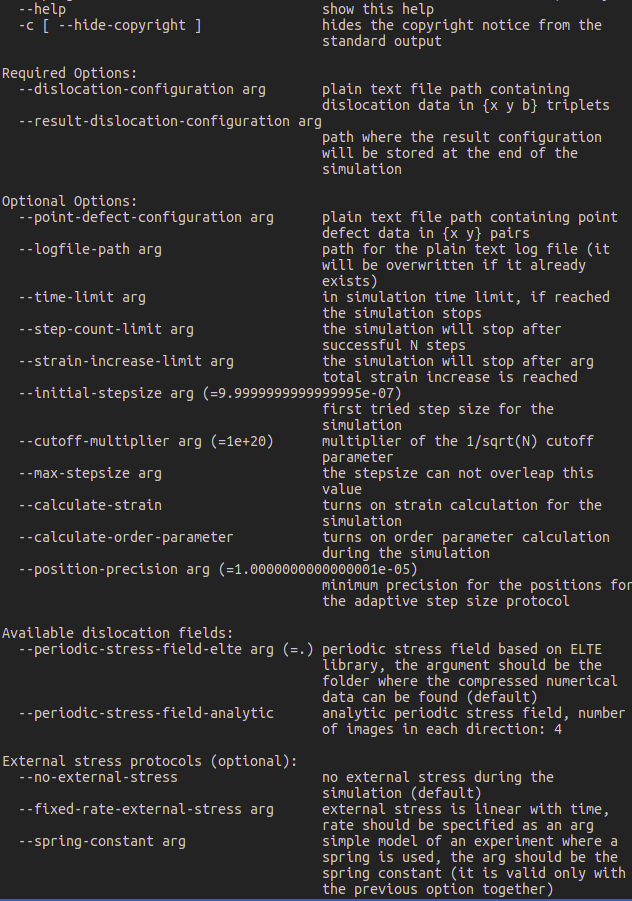
\includegraphics[width=0.65\columnwidth]{docs.png}
		\caption{Argument documentation}
	\end{figure}

	\subsection{Plotting the stress matrix - setup}

	\par I was able to extract the stress field around a dislocation
	in the origo. I extended the code with this functionality. The object oriented structure
	helped me to easily output the field to the standard file stream.

	\begin{lstlisting}[language=C++]{Name=test2}
	void PeriodicShearStressELTE::outPutStress(){

		float resolution = 0.005;
	
		for(float i = -0.5; i < 0.5; i += resolution){
			for(float j = -0.5; j < 0.5; j += resolution){
				fout << xy(i, j) << ";";
			}
			fout << "\n";
		}
	
	}
	\end{lstlisting}


	\par Where the function \textit{xy(double x, double y)} calculates the field around the dislocation
	at coordinates \textit{i, j} with a 0.005 resolution in a $-0.5, 0.5$ grid.

	\section{Visualization}
	\vspace{0.1cm}

	\par The visualization was a hard task as it is not a piece of cake to visualize
	stress fields that are varying on a high scale. The stress field contains some enormous and
	many tiny numerical values therefore it must be considered during visualization how to handle this.

	\par The $matplotlib$ package provides a clean interface to visualize such
	`images` on a symmetric logarithmic scale. This means that for a while the scale is linear
	but  after a given threshold it becomes logarithmic, it is also symmetric since
	the fields very from negative to positive values.

	I ran the code
	with different types of fields, such as the stress field code-named ELTE and
	several analytic fields. The analytic fields only differ in accuracy since they are
	calculated using N images.

	\par The ELTE field looks the following way:

	\begin{figure}[H]
		\centering
		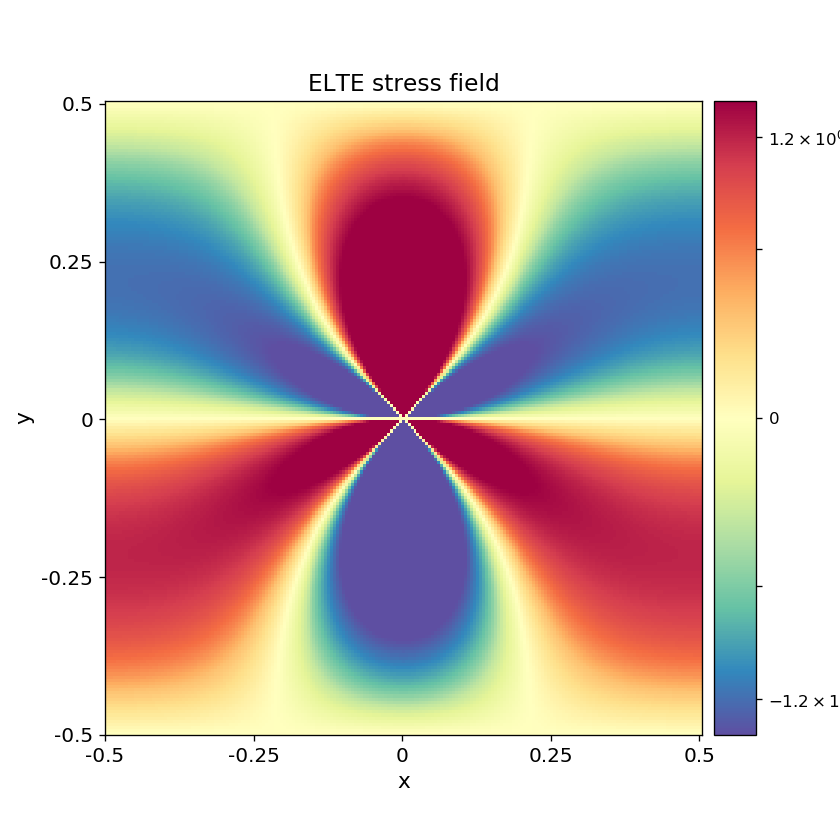
\includegraphics[width=0.4\columnwidth]{./elte_stress_field.png}
		\caption{Stress field visualization}
	\end{figure}

	\par While changing N from 1 to 12 in the calculation of analytic fields results are the
	following in order:

	\vspace{1cm}

	\begin{minipage}{0.22\columnwidth}
		\centering
		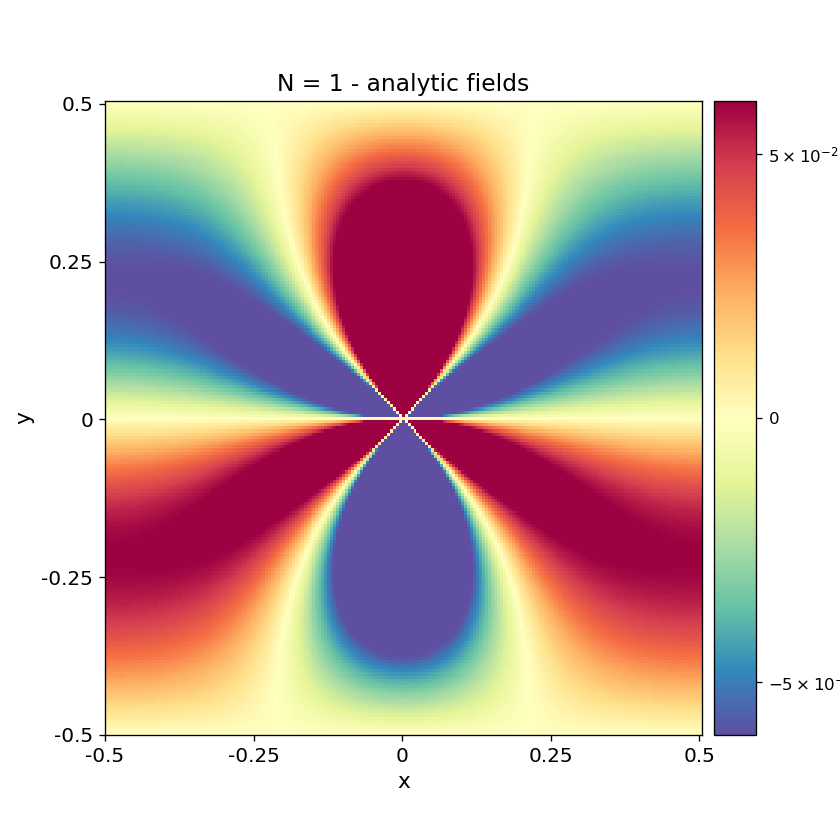
\includegraphics[width=\columnwidth]{./stress_field_01.png}
	\end{minipage}
	\begin{minipage}{0.22\columnwidth}
		\centering
		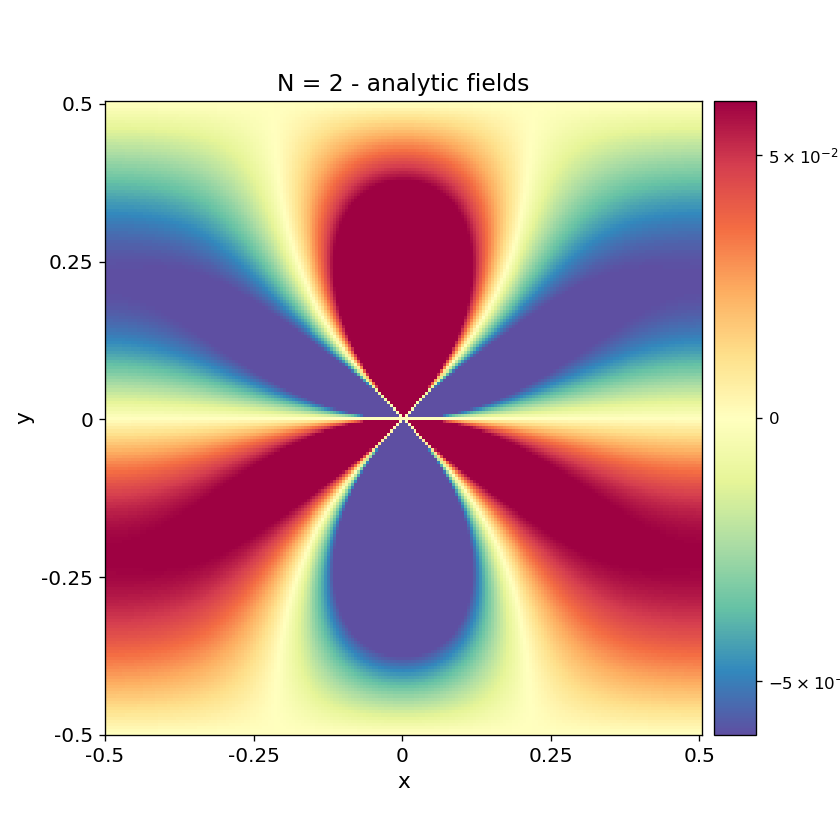
\includegraphics[width=\columnwidth]{./stress_field_02.png}
	\end{minipage}
	\begin{minipage}{0.22\columnwidth}
		\centering
		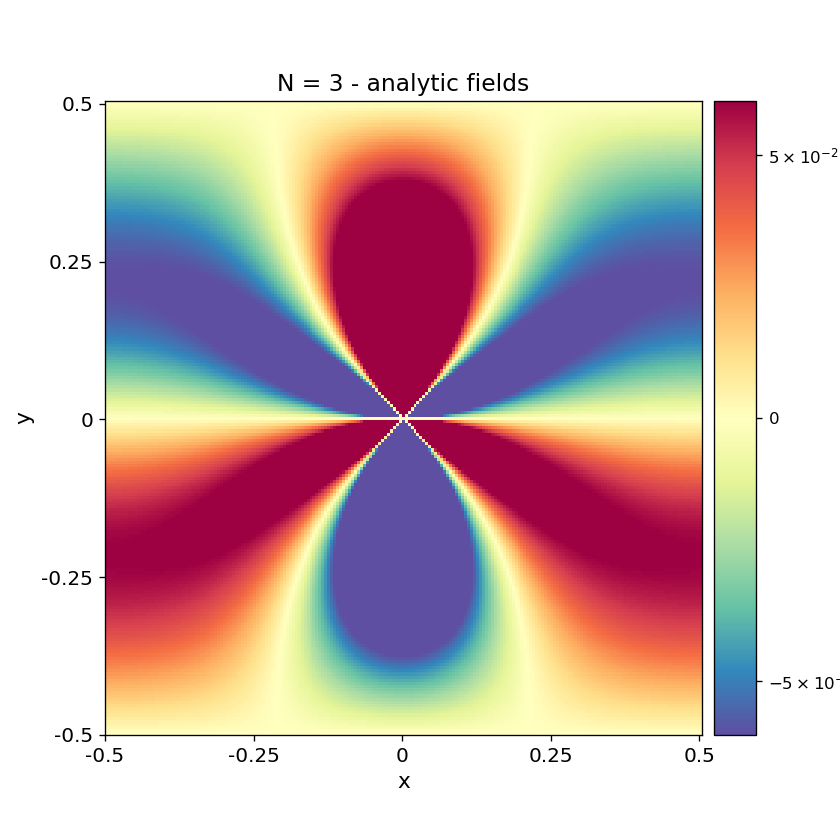
\includegraphics[width=\columnwidth]{./stress_field_03.png}
	\end{minipage}
	\begin{minipage}{0.22\columnwidth}
		\centering
		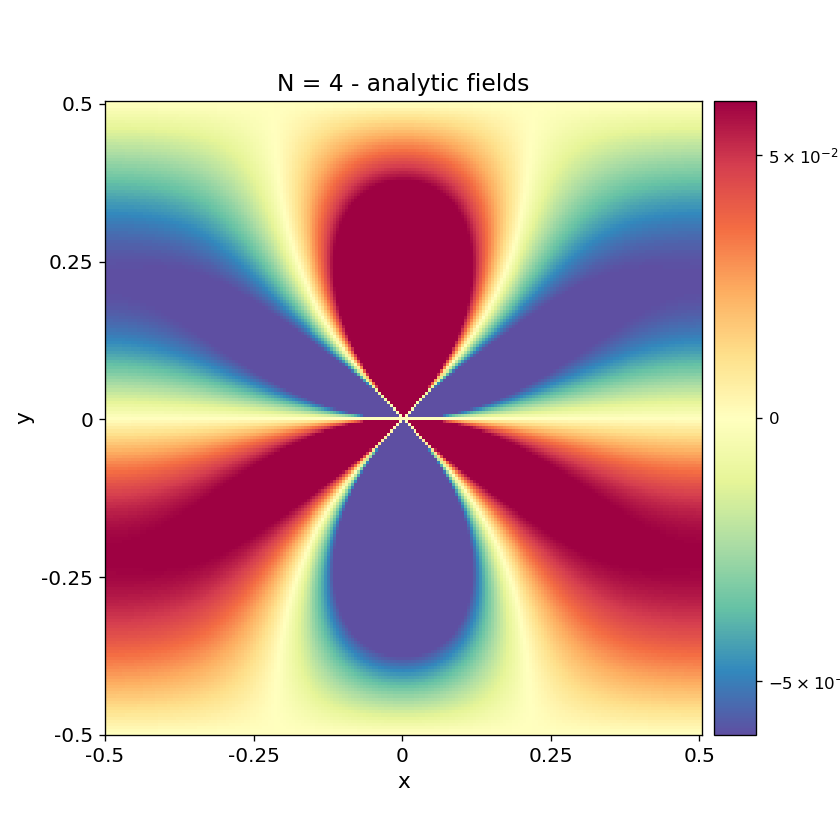
\includegraphics[width=\columnwidth]{./stress_field_04.png}
	\end{minipage}

	\begin{minipage}{0.22\columnwidth}
		\centering
		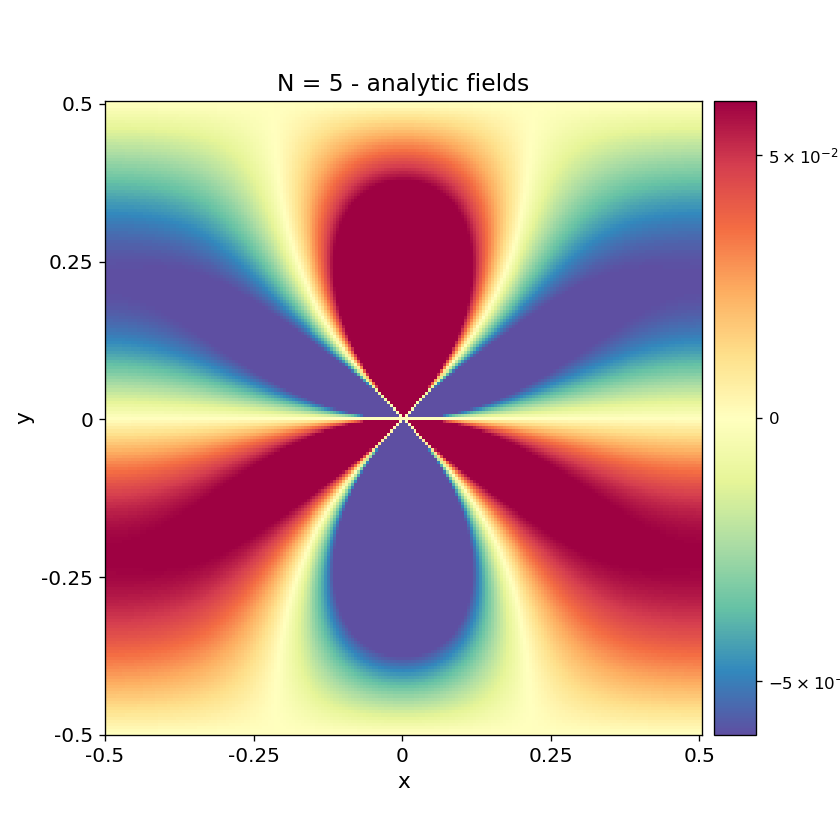
\includegraphics[width=\columnwidth]{./stress_field_05.png}
	\end{minipage}
	\begin{minipage}{0.22\columnwidth}
		\centering
		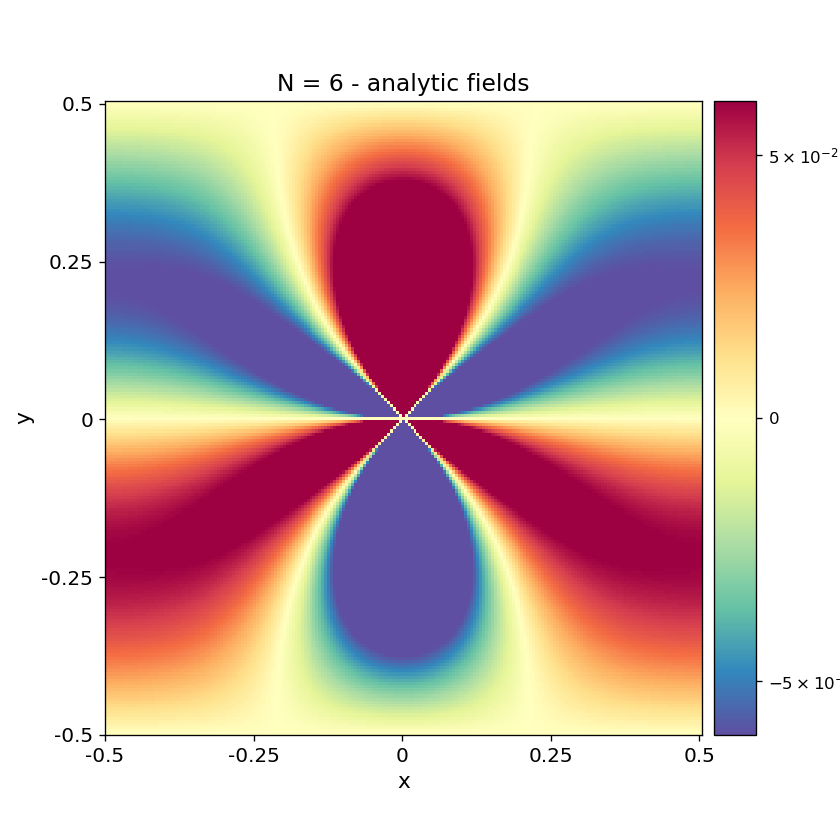
\includegraphics[width=\columnwidth]{./stress_field_06.png}
	\end{minipage}
	\begin{minipage}{0.22\columnwidth}
		\centering
		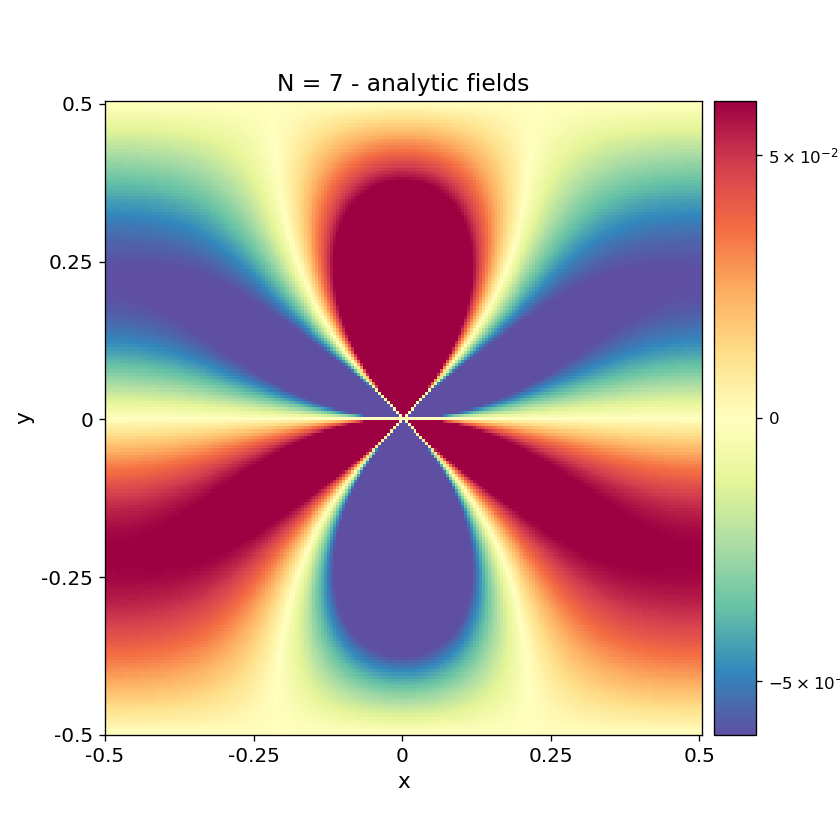
\includegraphics[width=\columnwidth]{./stress_field_07.png}
	\end{minipage}
	\begin{minipage}{0.22\columnwidth}
		\centering
		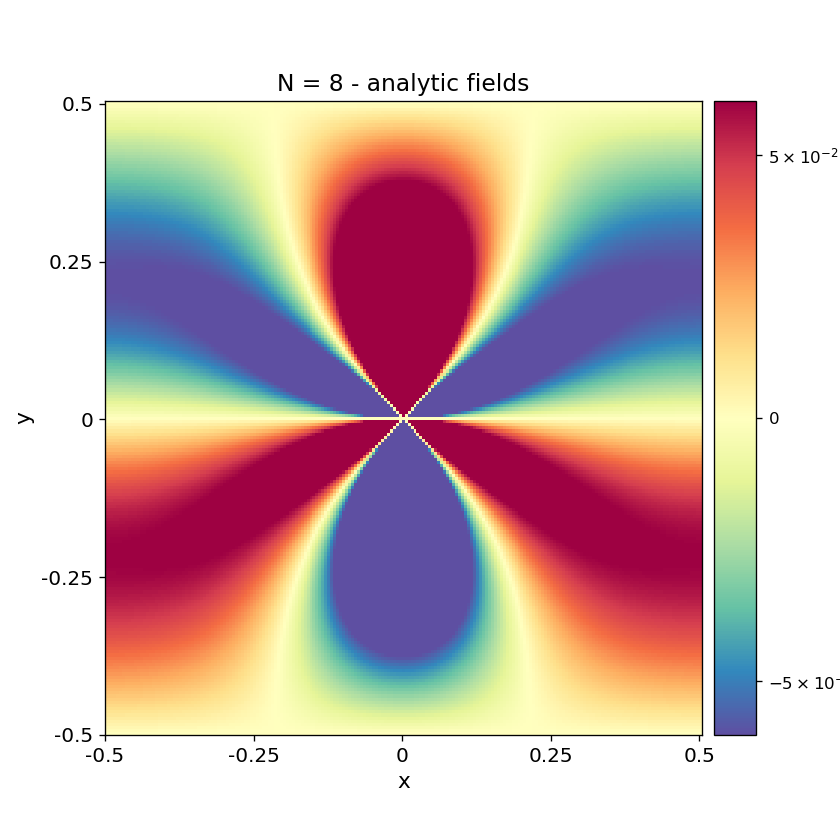
\includegraphics[width=\columnwidth]{./stress_field_08.png}
	\end{minipage}

	\begin{minipage}{0.22\columnwidth}
		\centering
		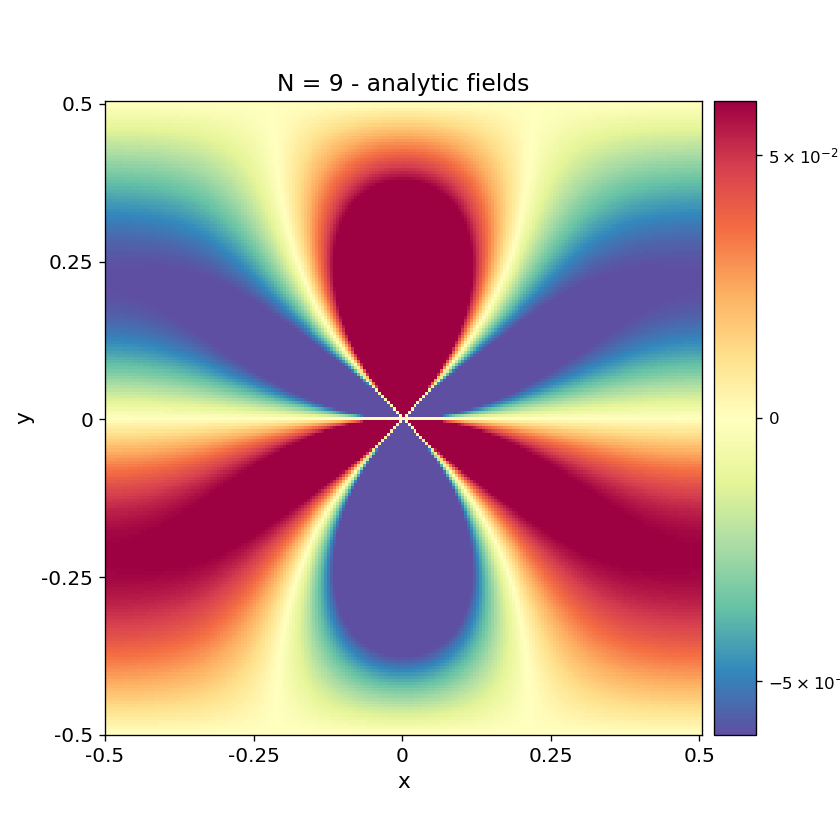
\includegraphics[width=\columnwidth]{./stress_field_09.png}
	\end{minipage}
	\begin{minipage}{0.22\columnwidth}
		\centering
		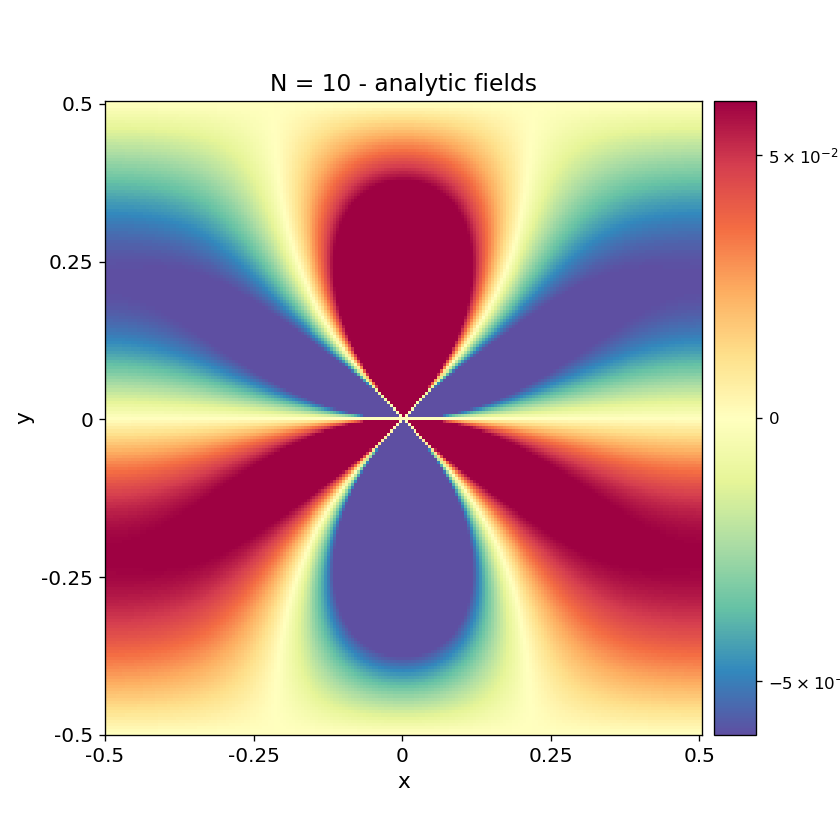
\includegraphics[width=\columnwidth]{./stress_field_10.png}
	\end{minipage}
	\begin{minipage}{0.22\columnwidth}
		\centering
		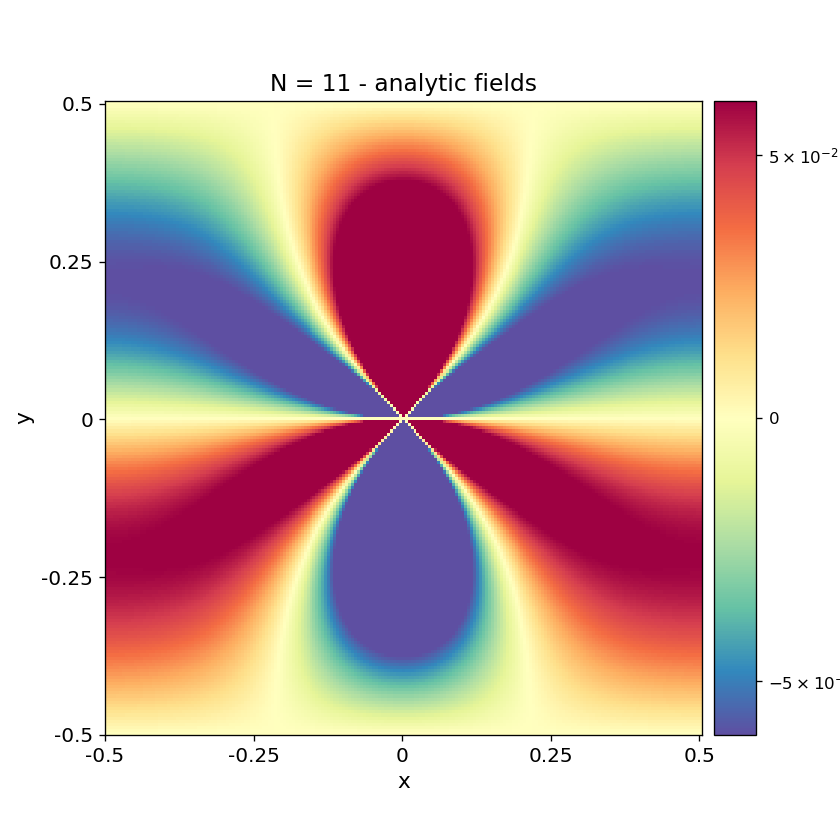
\includegraphics[width=\columnwidth]{./stress_field_11.png}
	\end{minipage}
	\begin{minipage}{0.22\columnwidth}
		\centering
		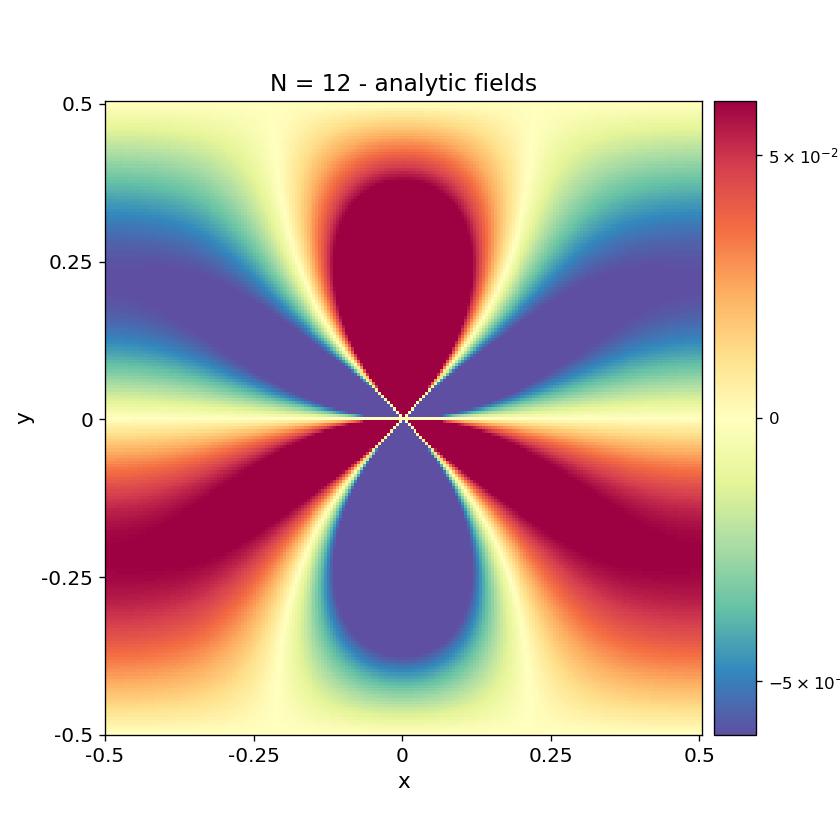
\includegraphics[width=\columnwidth]{./stress_field_12.png}
	\end{minipage}

	\vspace{1cm}

	\par The difference doesn't really show on the images but getting the
	consecutive differences of images and displaying that one can achieve
	much better visualization of the fields:

	\begin{figure}[H]
		\centering
		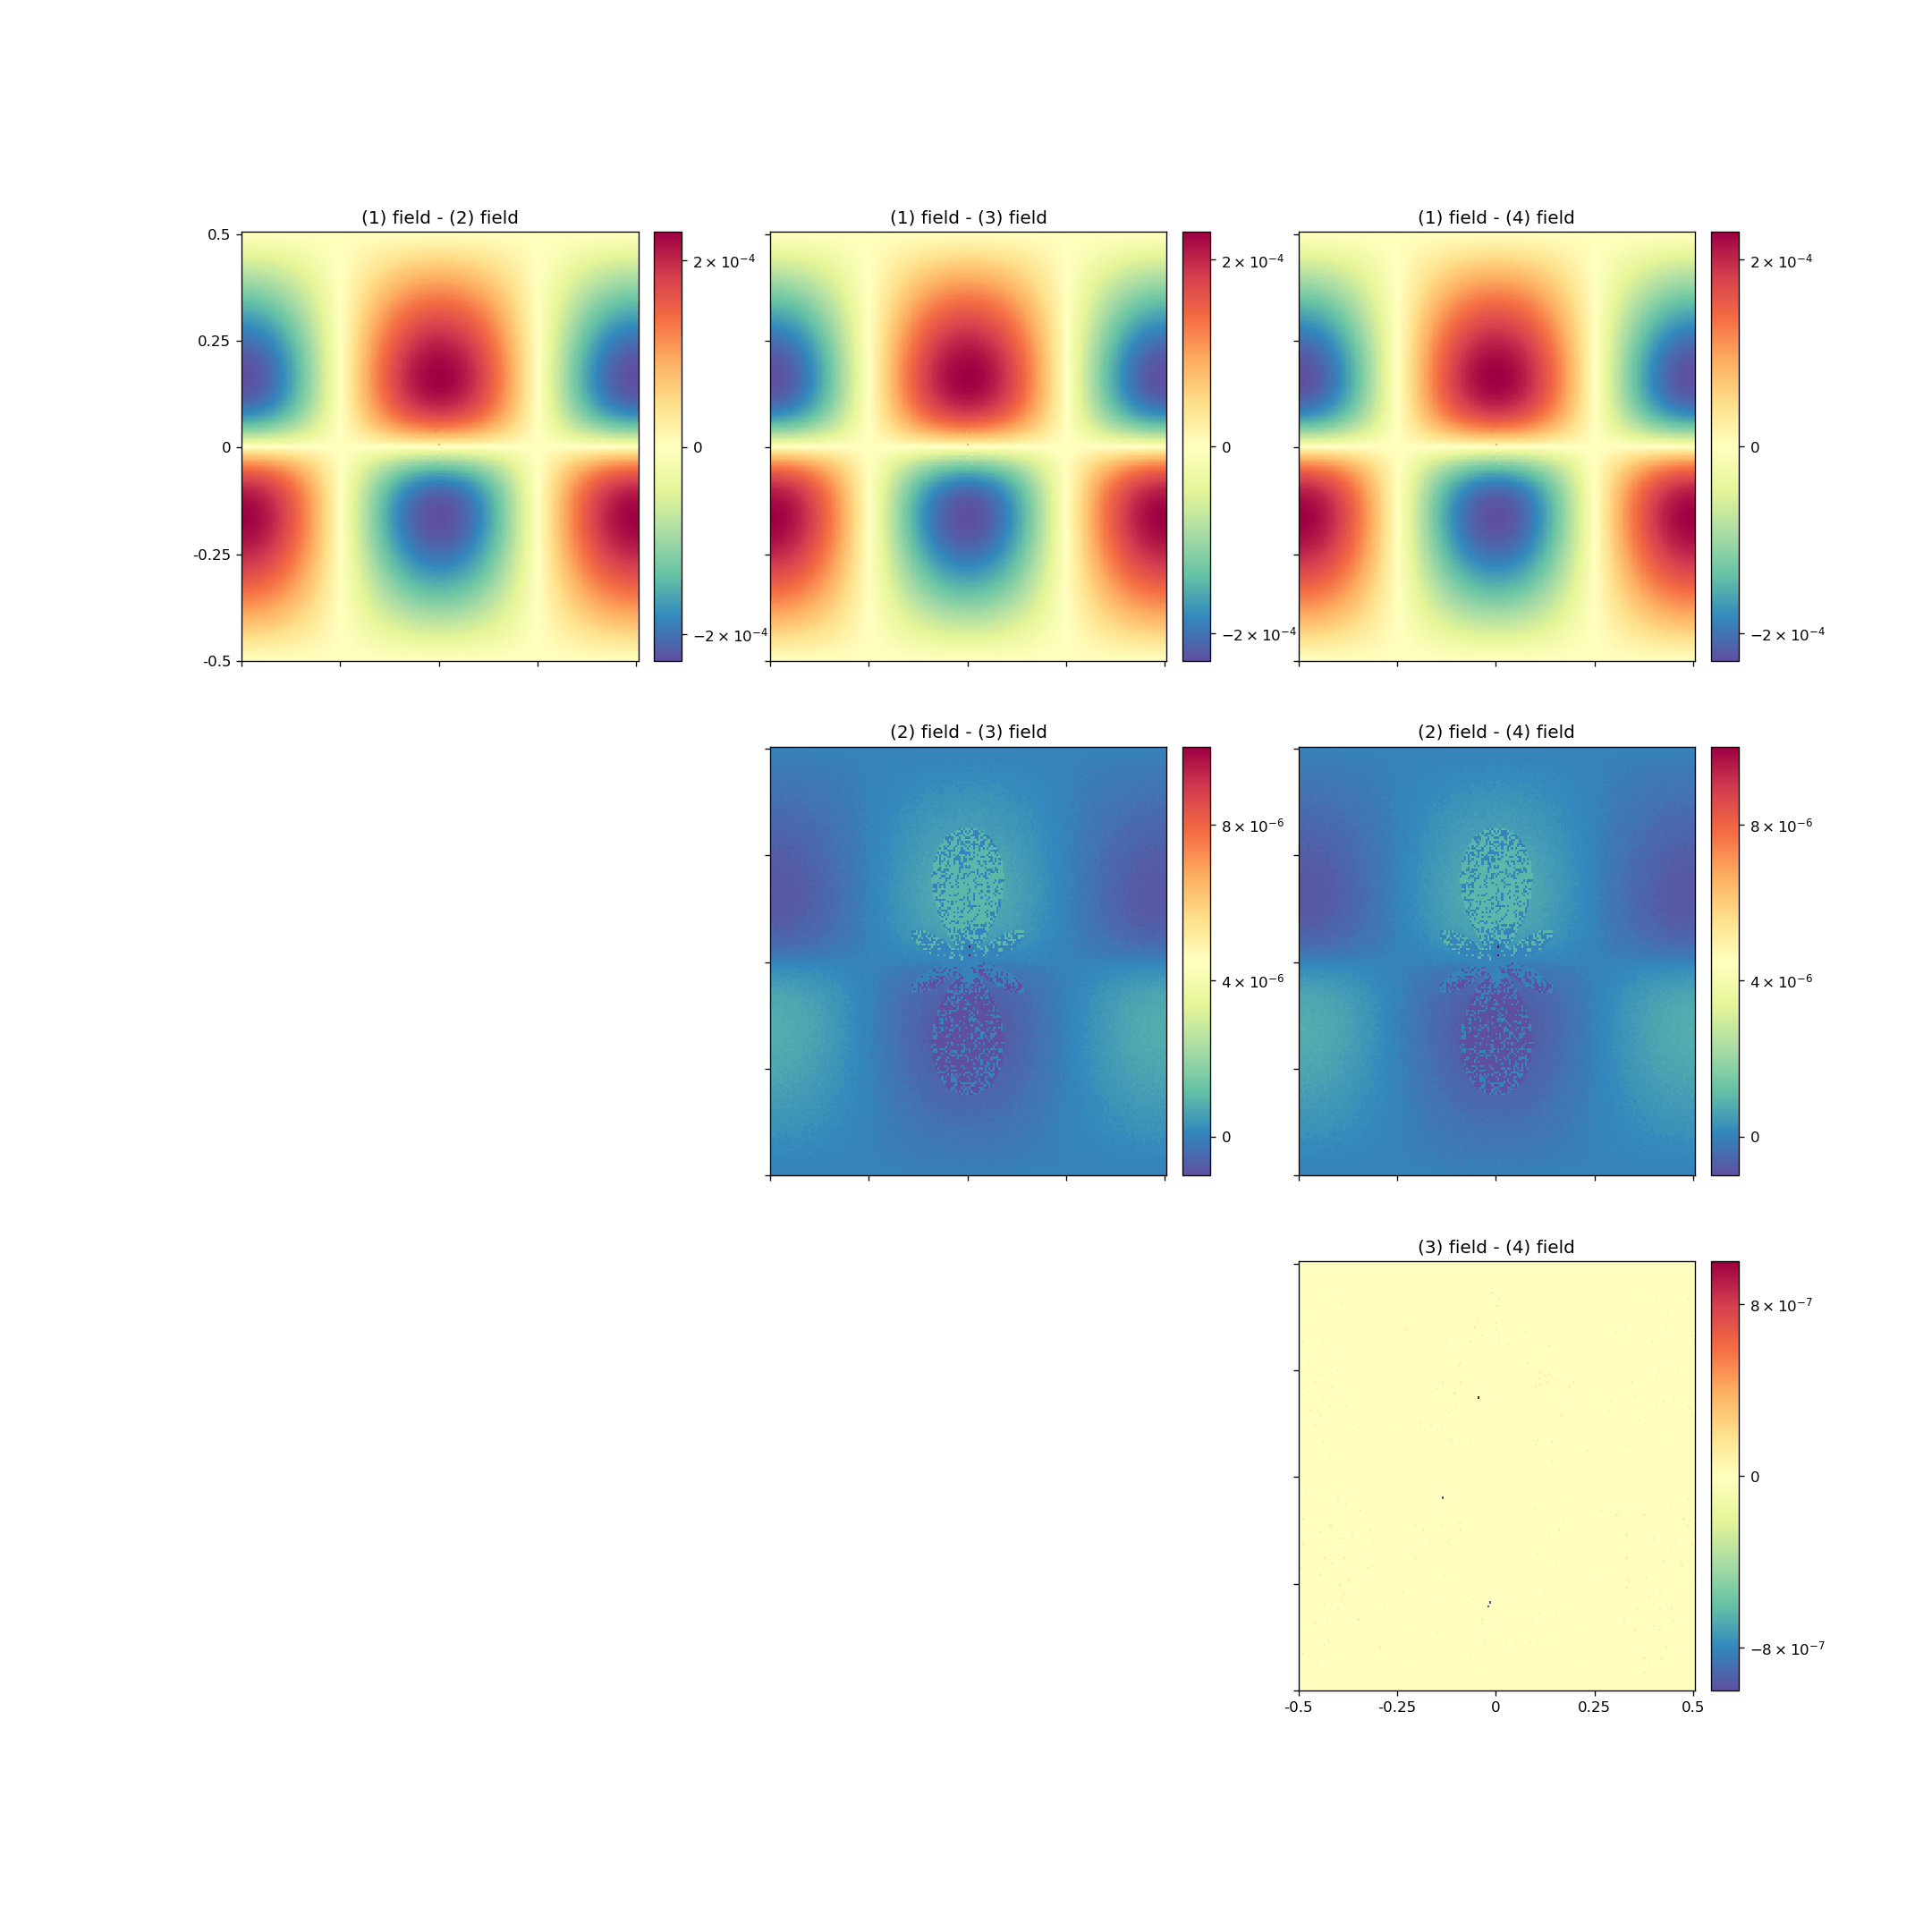
\includegraphics[width=.8\columnwidth]{./difference_of_analytic_fields.png}
		\caption{Difference of analytic fields}
	\end{figure}

	\par Where row - column ordering is created. It can be seen that the very last plot,
	that shows the difference between the 3rd and 4th analytic fields, where N=4 or N=3.
	It can be clearly seen that disregarding some points the analytic fields become equal from N=3
	and therefore the difference is almost everywhere zero.

	\vspace{1cm}

	\par Having plotted the difference of analytic fields I moved on with
	showing the differences of analytic and ELTE code-named stress fields.

	\begin{figure}[H]
		\centering
		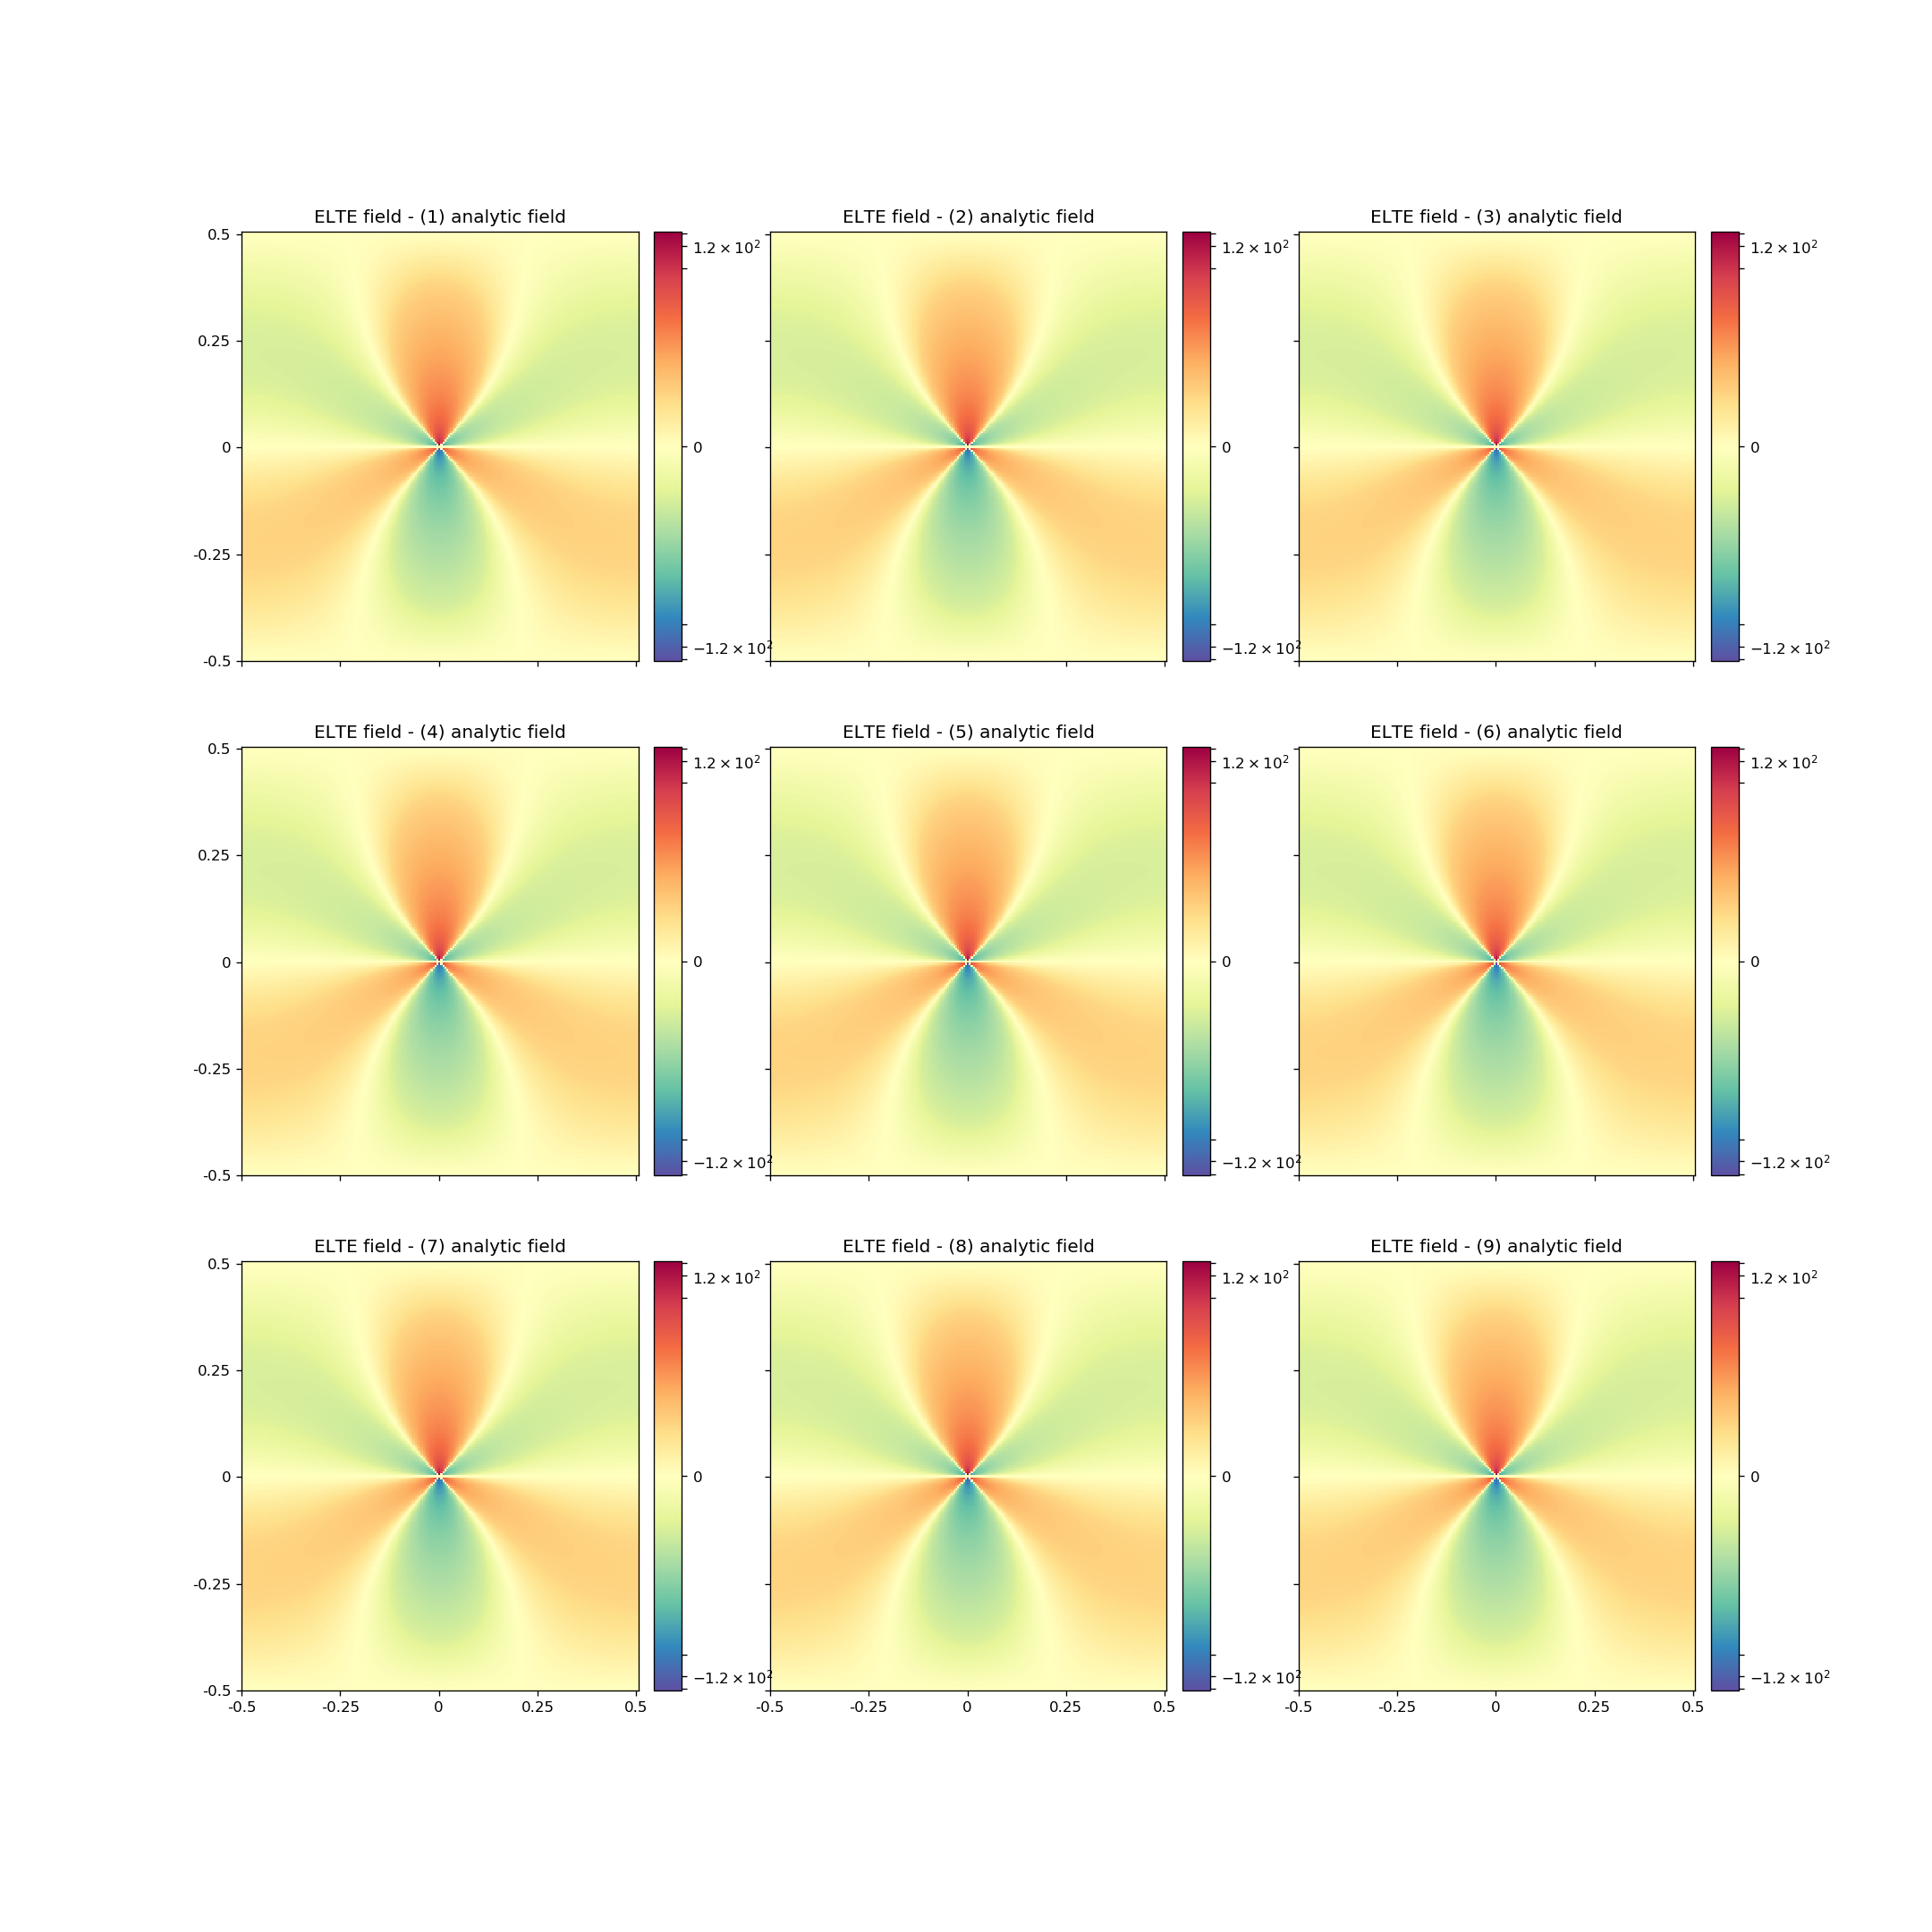
\includegraphics[width=.8\columnwidth]{./difference_of_analytic_field_and_elte_field.png}
		\caption{Difference with the ELTE field}
		\label{fig:elte}
	\end{figure}

	\par From this plot it can be derived that they are equal almost everywhere but in the middle where
	they differ mostly.

	\section{Numeric analysis of different stress fields}

	\par Moving on to the log file that is produced after each simulation I had to create
	a random dislocation configuration with 64 dislocations to feed in for the numerical tests.

	\par The log file contains the following information:

	\begin{itemize}
		\item simulation time
		\item number of successful steps
		\item number of failed steps
		\item worst error ratio squared
		\item average speed of the dislocations
		\item cutoff (used in the semi implicit scheme)
		\item order parameter
		\item value of the external stress
		\item computation time between the last two successful steps
		\item accumulated strain
		\item average v2
		\item energy of the system
	\end{itemize}

	\par Where I considered the average speed, average speed squared and energy variables in the function of time
	as relevant variables to test the system numerically.

	\par The energy is better described as the energy loss of the system since the system equilibrates
	and loses energy.

	\par I also saved the output dislocation file where I get the
	resulting dislocation coordinates but it is not interesting since it cannot
	be decided which point corresponds to which starting location.

	\begin{figure}[H]
		\centering
		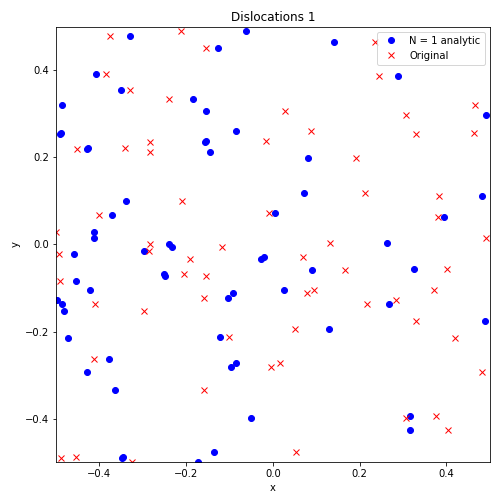
\includegraphics[width=0.4\columnwidth]{Dislocations1.png}
		\caption{Starting and finishing dislocation location distribution}
	\end{figure}

	\par Previously I mentioned that the analytic field is calculated via taking into account N images.

	\begin{itemize}
		\item in the y-axis the periodic boundary condition can be analytically calculated by summing up infinitely many fields
		\item in the x-axis N images must be taken into account when the summation of fields is executed since there is no analytic formula
		\item it can be imagined as field stacking in the x-axis, when a dislocation crosses the simulation boundary on the right hand side it enters the same field stacked after the previous one on the left hand side, therefore the same field acts upon it
	\end{itemize}

	\begin{equation*}
		\sigma_{xx} = \frac{-Gb}{2\pi(1-\nu)}\frac{y(3x^{2} + y^{2})}{(x^{2} + y^{2})^{2}}
	\end{equation*}

	\begin{equation*}
		\sigma_{yy} = \frac{Gb}{2\pi(1-\nu)}\frac{y(x^{2} - y^{2})}{(x^{2} + y^{2})^{2}}
	\end{equation*}

	\begin{equation*}
		\tau_{xy} = \frac{Gb}{2\pi(1-\nu)}\frac{x(x^{2} - y^{2})}{(x^{2} + y^{2})^{2}}
	\end{equation*}

	\vspace{0.2cm}

	\par The off diagonal part is used in the simulation.

	\par The previously seen ELTE stress field \ref{fig:elte} which has a periodic boundary condition.

	\begin{figure}[H]
		\centering
		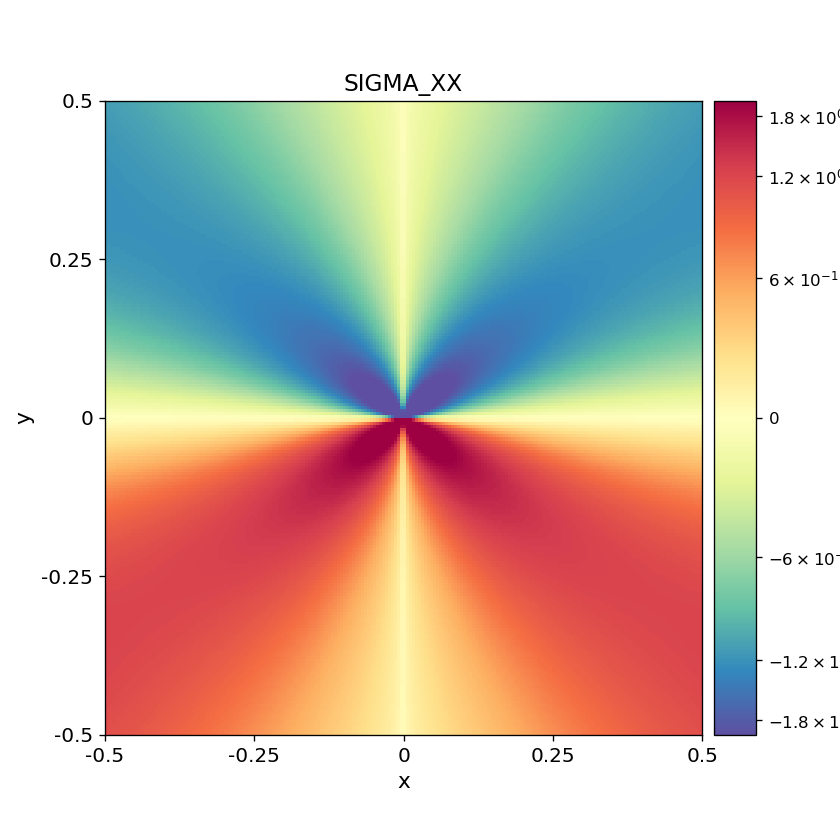
\includegraphics[width=0.4\columnwidth]{elte_stress_field_SIGMA_XX.png}
		\caption{Theoretical $\sigma_{xx}$ component}
	\end{figure}

	\begin{figure}[H]
		\centering
		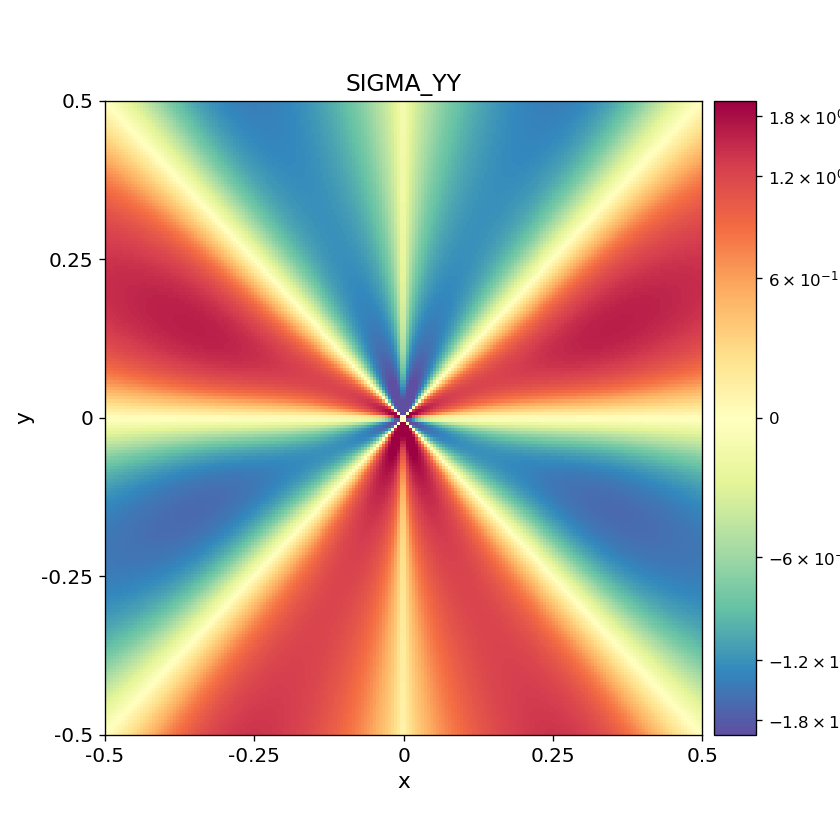
\includegraphics[width=0.4\columnwidth]{elte_stress_field_SIGMA_YY.png}
		\caption{Theoretical $\sigma_{yy}$ component}
	\end{figure}

	\begin{figure}[H]
		\centering
		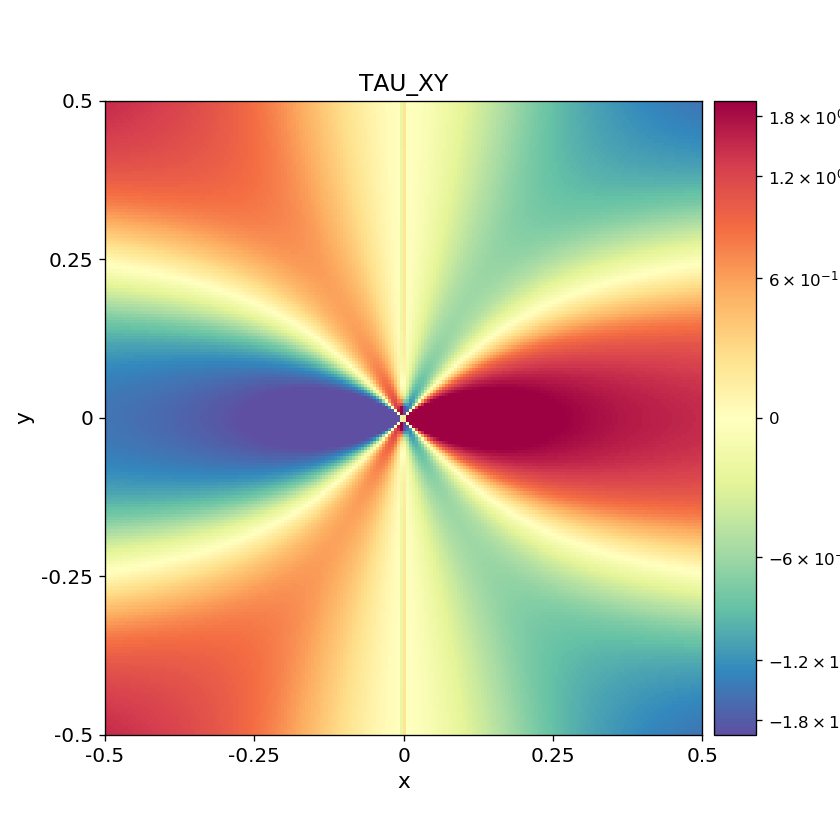
\includegraphics[width=0.4\columnwidth]{elte_stress_field_TAU_XY.png}
		\caption{Theoretical $\tau_{xy}$ component}
	\end{figure}

	\par This resembles to the ELTE field as it should, since the off-diagonal
	components are were displayed previously by my visualization programs.

	\begin{minipage}[t]{0.42\columnwidth}
		\centering
		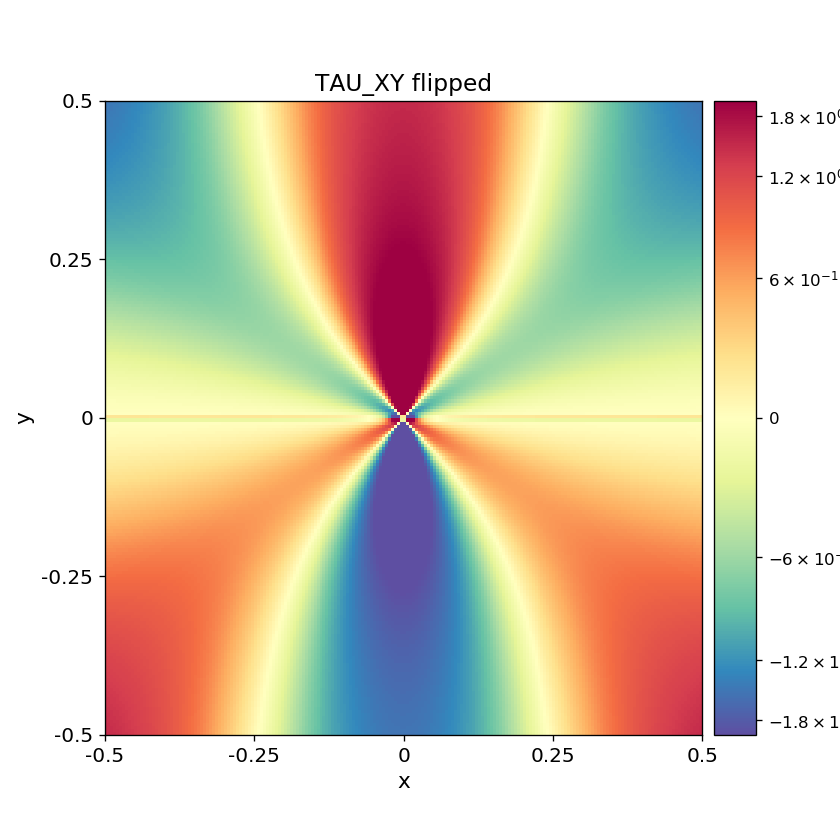
\includegraphics[width=0.8\columnwidth]{elte_stress_field_TAU_XY_flipped.png}
	\end{minipage}
	\begin{minipage}[t]{0.42\columnwidth}
		\centering
		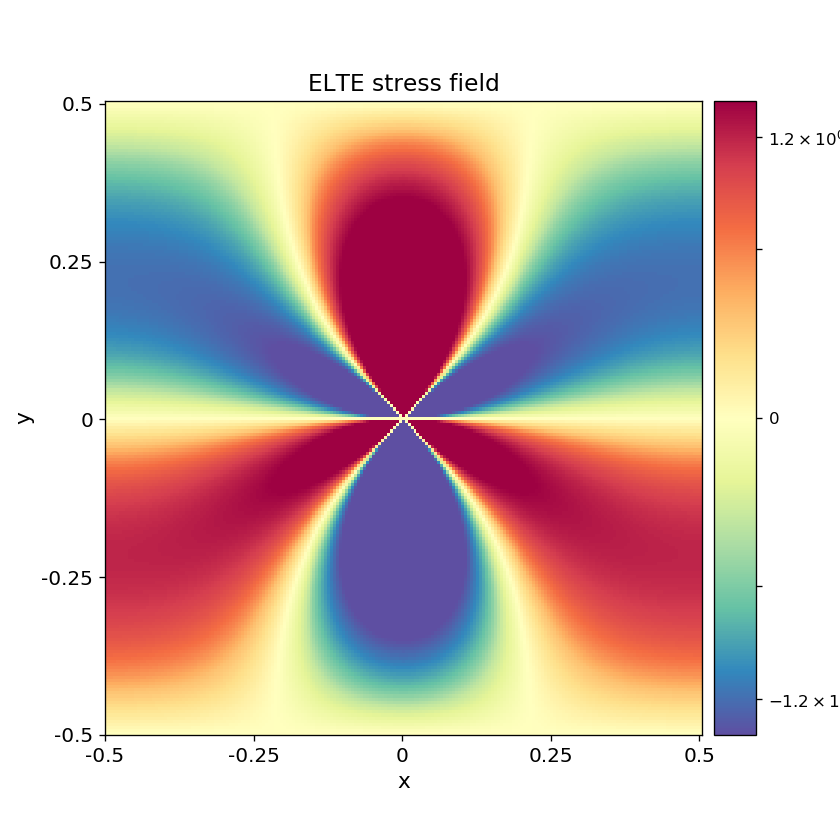
\includegraphics[width=0.8\columnwidth]{elte_stress_field.png}
	\end{minipage}

	\par The ${\tau}^{T}_{xy}$ component and the ELTE field.

	\subsection{Analysis conclusion}

	\par Analyzing the log files and comparing them the following can be deduced:

	\begin{figure}[H]
		\centering
		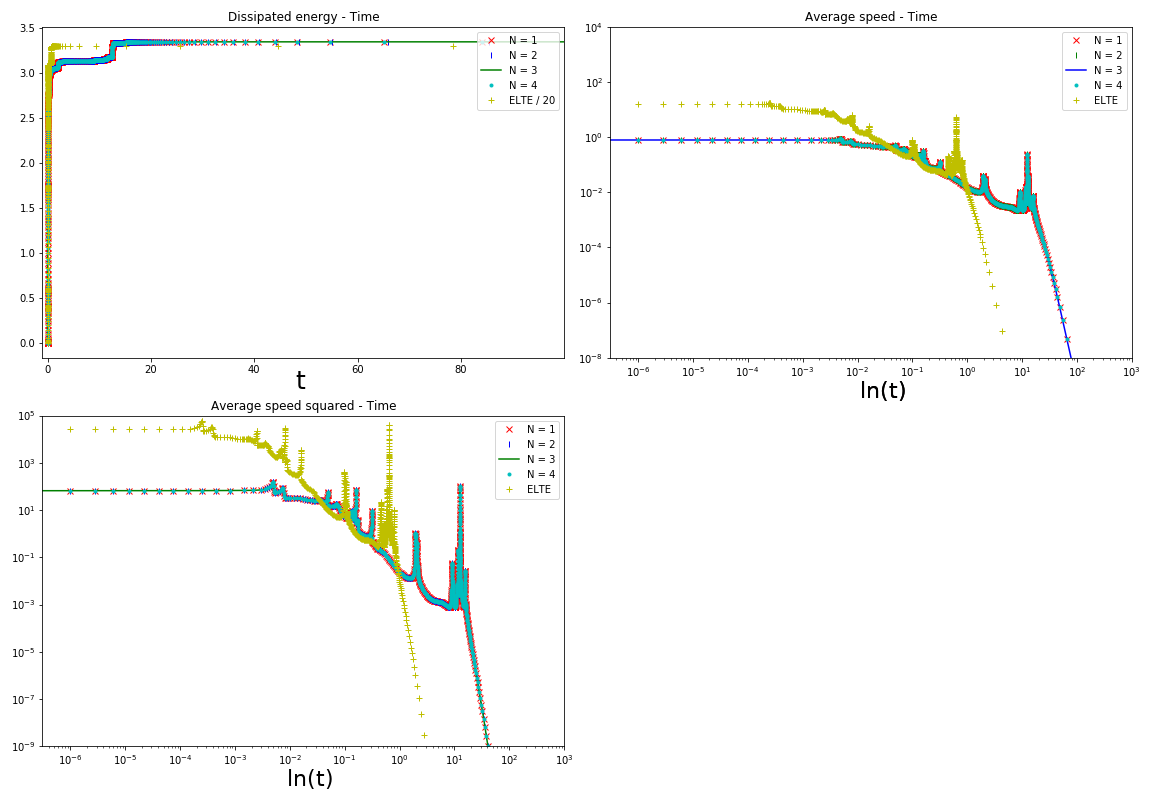
\includegraphics[width=0.95\columnwidth]{all.png}
	\end{figure}

	\begin{itemize}
		\item The ELTE field dissipates energy faster than the analytic fields which do not differ that much.
		\item It is worth considering why we see peaks on the speed diagrams. It is due to dislocations getting close to each other and repenting each other with an immense force resulting in high velocity peaks.
		\item Otherwise the same structure can be seen on both systems.
	\end{itemize}

	\section{Averaged inputs analysis}

	\par After having acquired the previous results I could move on with feeding
	the algorithm with 10 different dislocation setups each containing 64 dislocations
	randomly generated in a $-0.5$, $0.5$ grid in the x-y plane.

	\par All the systems ran for different times. Due to this averaging was not straightforward
	at all I needed to find the lowest one and average until that one, which ran for $\approx$ 1033.7
	time-steps defined by the simulation.

	\par I plotted these results as I did previously:

	\begin{figure}[H]
		\centering
		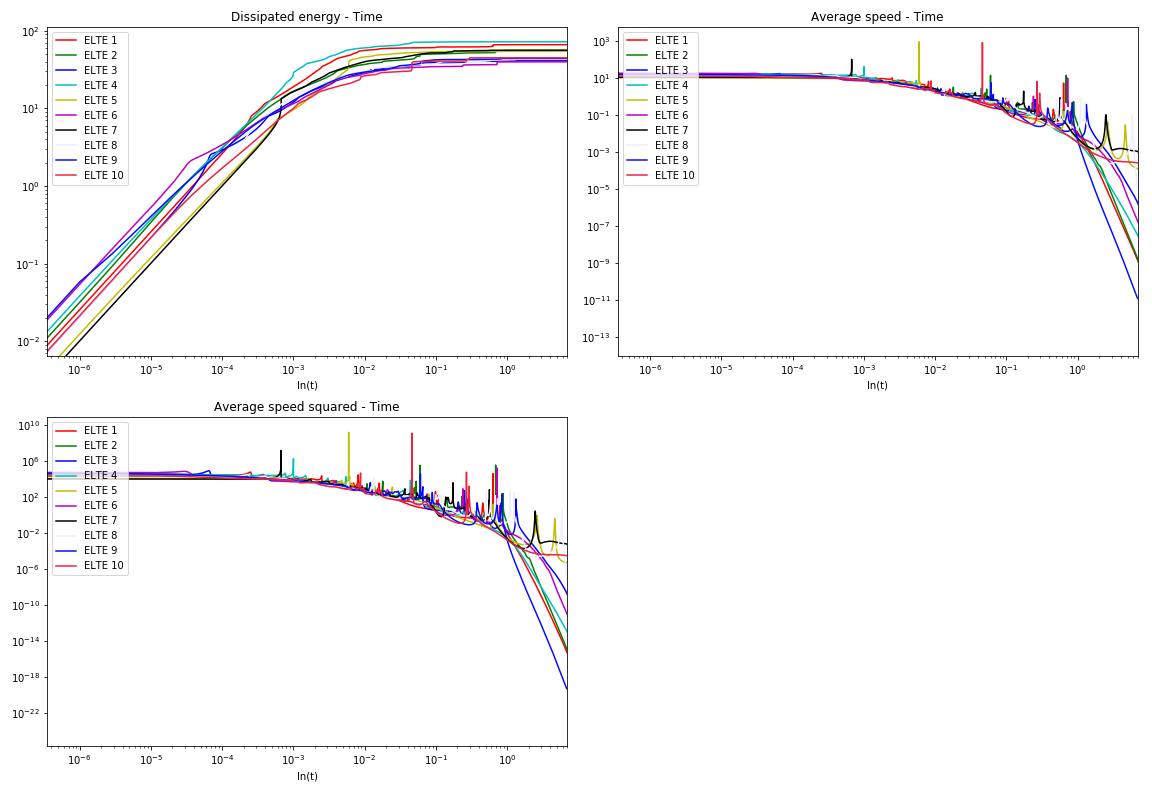
\includegraphics[width=0.99\columnwidth]{all_elte.png}
		\caption{Each line is a different run with a different input file with the ELTE stress field applied}
	\end{figure}

	\par Averaging them took some effort since not all output files had the same row count since
	time-steps are defined, not time therefore the systems evolve for different but similar
	time periods. I took the shortest one and avaraged based on the length of that.

	\begin{figure}[H]
		\centering
		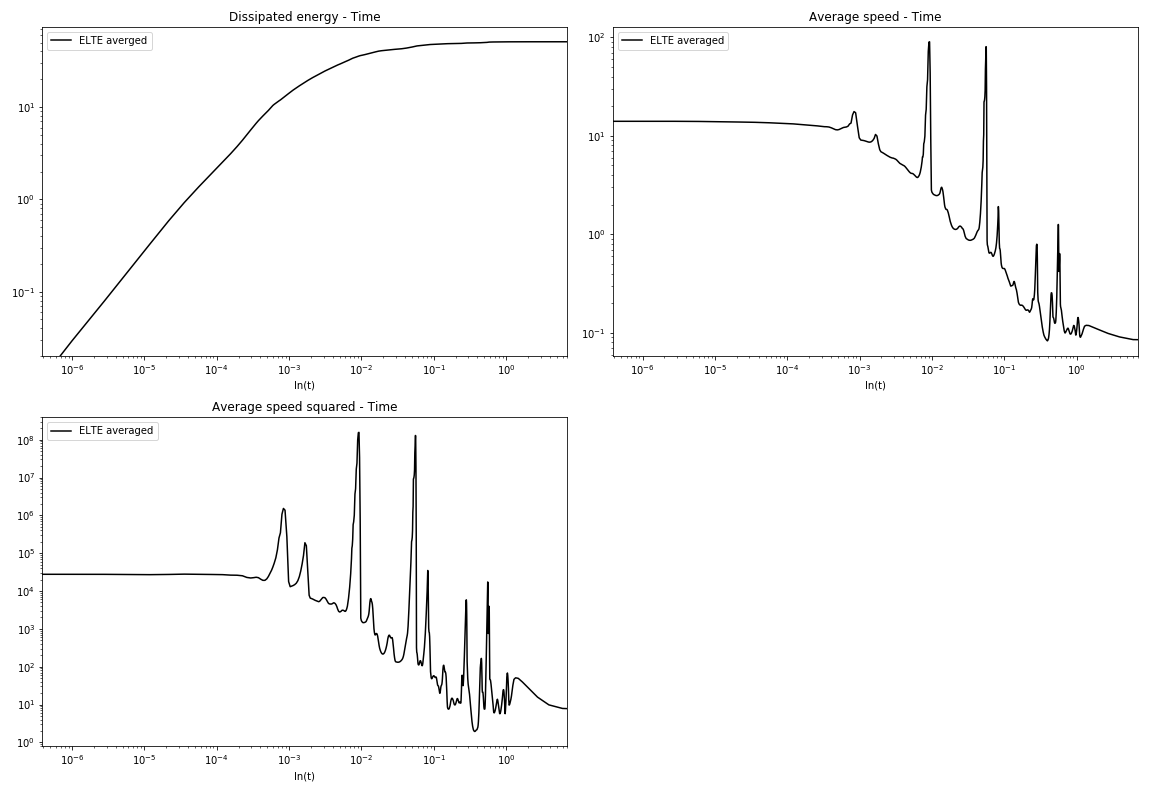
\includegraphics[width=0.99\columnwidth]{all_elte_averaged.png}
		\caption{Ten averaged simulations with ELTE field applied}
		\label{fig:avg}
	\end{figure}

	\subsection{Analysis conclusion}

	\par Generally it seems like the system doesn't depend much on
	the actual dislocations' and they all behave very similarly. Averaging
	more simulations would result in peaks disappearing on \ref{fig:avg} and only the dissipating
	tendency could be seen.

	\section{Experimenting with external stress}

	\par There is one external stress protocol defined, so far none was used in the previous simulation
	runs. A fixed rate external stress can be applied and its value defined as an input parameter.

	\par The provided input file for these runs was an earlier output from an equilibrated system.

	\par I ran two set-ups with external stress set to $0.1$ and $0.01$. Everything is dimensionless
	in the simulation so therefore they only have numeric number, but 0.1 is large and 0.01 is not so large.

	\par I run the numerical analysis on these log files as well.

	\begin{figure}[H]
		\centering
		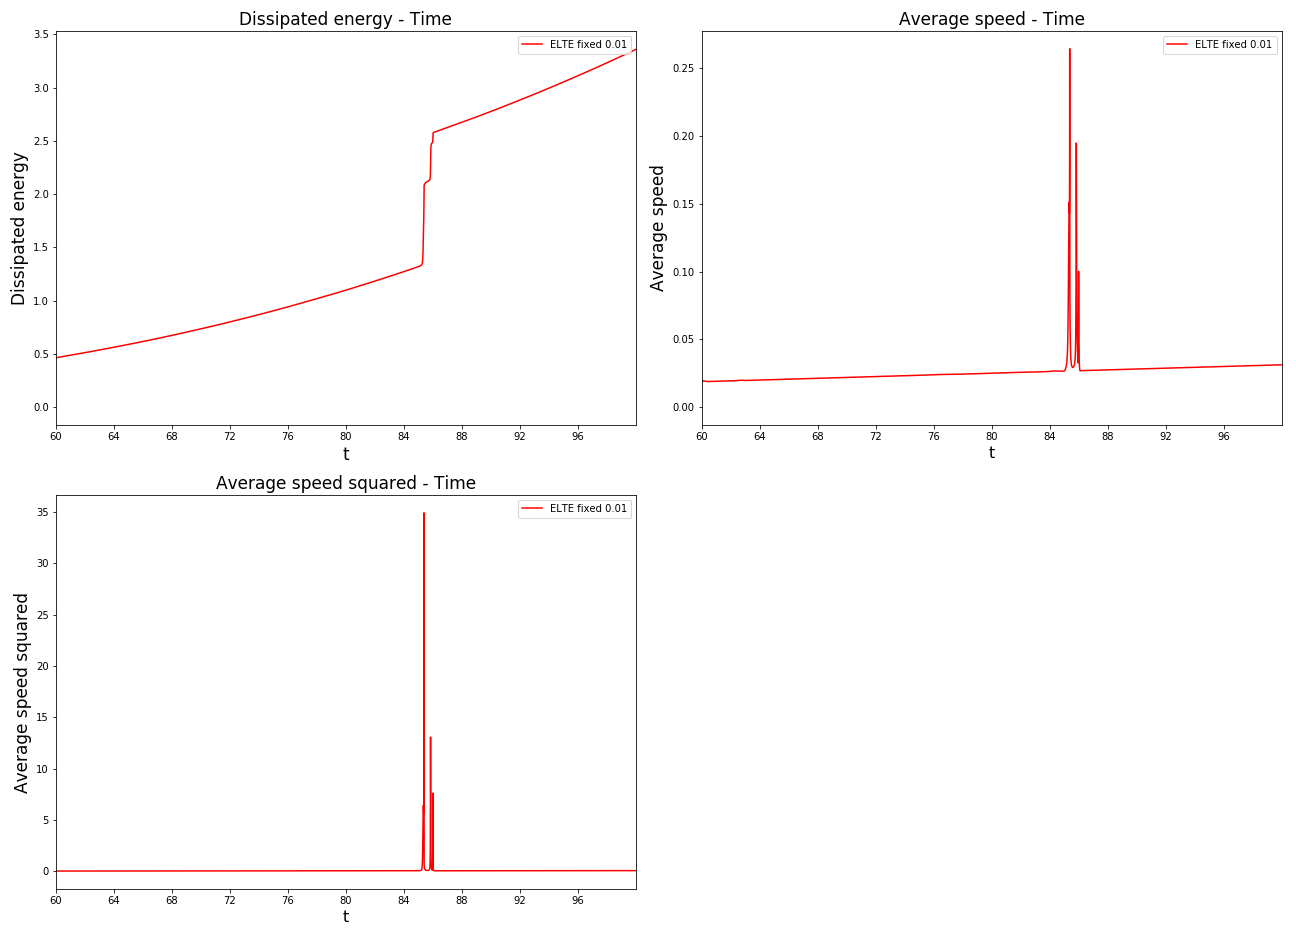
\includegraphics[width=0.99\columnwidth]{all_elte_fixed_0_0_1.png}
		\caption{Fixed stress rate - $0.01$}
	\end{figure}

	\par It can be seen that the system keeps on dissipating energy while time goes on
	on a fixed rate on log scale, therefore exponentially more on linear scale. Average
	speed and speed squared as well.

	\par Raising the external stress results in strange behavior.

	\begin{figure}[H]
		\centering
		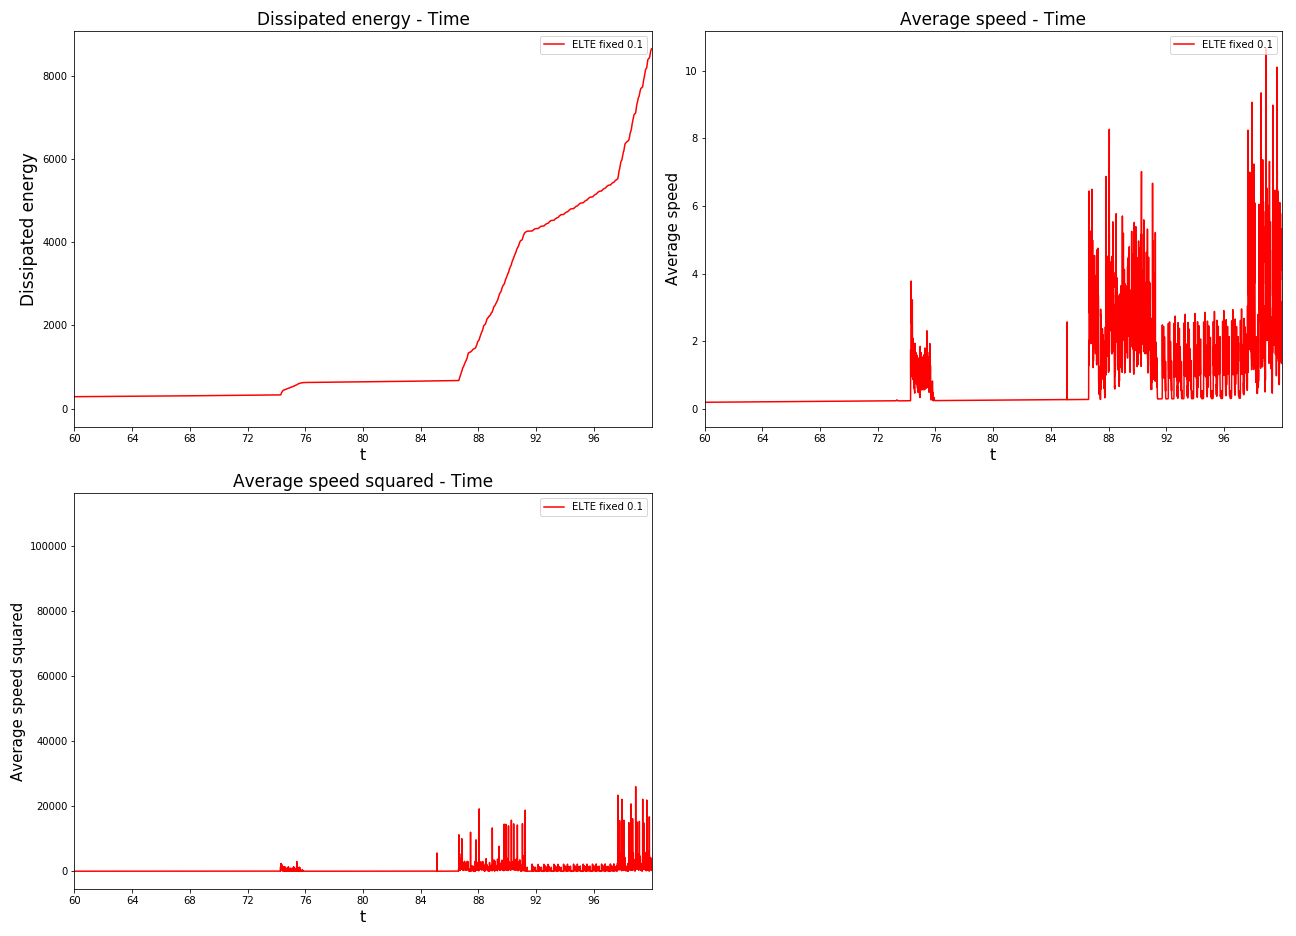
\includegraphics[width=0.99\columnwidth]{all_elte_fixed_0_1.png}
		\caption{Fixed stress rate - $0.1$}
	\end{figure}

	\par The interesting peaks can be the result of the system starting to behave
	as a fluid. I only show the regions on both figures which are interesting in this
	regerd.

	\subsection{Average distance test}

	\par Given a constant external stress the dislocations should get on average closer
	to each other. At each step I extracted the average of minimum pair distances. Meaning that at each step
	I calculated the minimum pair distances for each dislocation and output the average of that to
	the standard output.

	\par I used the ELTE stress field, with a $0.01$ external field applied and ran
	the simulation on 32, 64, 128 random dislocation sets.

	\par I ran them through a simulation to relax the input system and then provided the randomly
	generated data as input to the external stress applied run.

	\par The system containing 32 dislocations ran fast for long maximum time but the one with 64 and 128 were slow to run
	for even a $100$ limit simulation time.

	\begin{figure}[H]
		\centering
		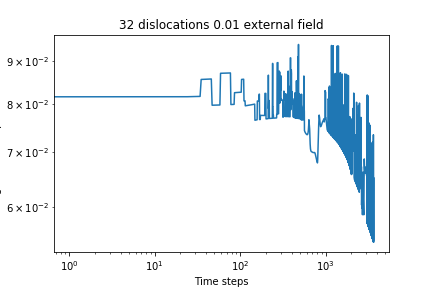
\includegraphics[width=0.8\columnwidth]{./32.png}
		\caption{System with 32 dislocations}
		\label{fig:32}
	\end{figure}

	\par On this figure \ref{fig:32} it can be evaluated easily that the average minimum distances
	are lowering while there are still these wiggly peaks. These are the result of the following effect:
	some particles are repenting others are attracting each other due to the force they can get so close
	to each other that they 'jump through' each other and start to repent/attract. When two or more
	dislocations reach this point these avalance like structures can be observed.

	\par With bigger system sizes data grow fast and time did not increase that much while this
	minimum pair distance lowered less significantly.

	\begin{figure}[H]
		\centering
		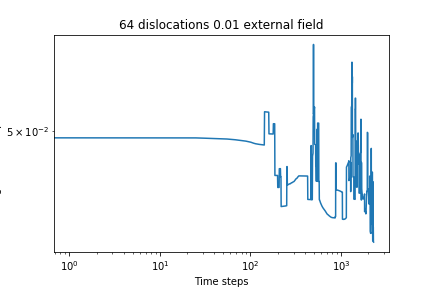
\includegraphics[width=0.8\columnwidth]{./64.png}
		\caption{System with 64 dislocations}
	\end{figure}

	\begin{figure}[H]
		\centering
		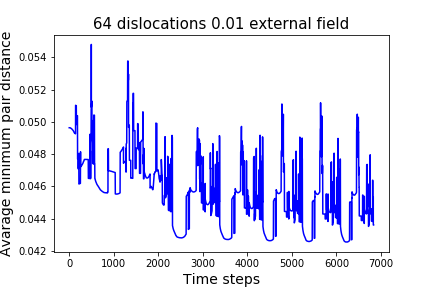
\includegraphics[width=0.8\columnwidth]{./64_long.png}
		\caption{System with 64 dislocations}
		\label{fig:64}
	\end{figure}

	\par Where \ref{fig:64} is run for significantly longer (for twice the amount of original run time $100$ provided).
	Lowering can be seen on these figures but with an expanding system size wiggliness
	is worsening. The periodic condition can be evidently seen in \ref{fig:64} as particles repent each
	other but due to the periodic boundary condition they get close to each other again and again.

	\par With a 128 system size the expected behavior cannot be evidently seen.

	\begin{figure}[H]
		\centering
		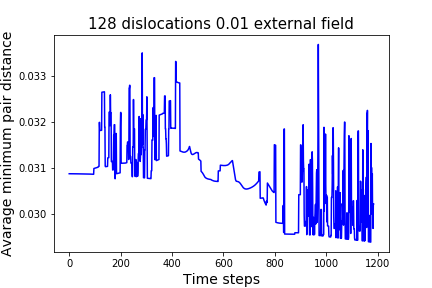
\includegraphics[width=0.8\columnwidth]{./128.png}
		\caption{System with 128 dislocations}
	\end{figure}

	\section{Final conclusions}

	\par For these few weeks I got acquainted with the SDDDST package and its nooks and crannies.
	I created several visualizations and extended the code to acquire the required
	output. I also analyzed log files and tested the code's integrity. Not forgetting to mention
	that I did this in half the amount of the planned time.

	\par I also contacted my supervisor several times in person and in mail as well. My progress
	and results were clear for all the time being and I always asked when I got stuck.

	\par I consider my initial goal - finishing early successful and in general I consider this
	lab useful for those who weren't able to develop self discipline until now to
	be capable of meeting due dates.

	\bibliographystyle{unsrt}

	\bibliography{references}

\end{multicols*}
\end{document}